\documentclass {article}
\usepackage{amsmath}
\usepackage{appendix}
\usepackage{hyperref}
\hypersetup{
    colorlinks=true, % make the links colored
    linkcolor=black, % color TOC links in black
    urlcolor=red, % color URLs in red
    linktoc=all % 'all' will create links for everything in the TOC
}
\usepackage{float}
\usepackage{graphicx}
\graphicspath{{images/}}
\usepackage{csquotes}
\usepackage{fancyvrb}

\usepackage[backend=bibtex,style=numeric]{biblatex}
\addbibresource{sources.bib}


\usepackage{listings}
\lstset{
basicstyle=\small\ttfamily,
columns=flexible,
frame=single,
breaklines=true,
language=C++,
keywordstyle=\color{magenta}\ttfamily,
stringstyle=\color{red}\ttfamily,
commentstyle=\color{blue}\ttfamily,
}

\usepackage{tikz}
\usetikzlibrary{arrows}

\title {
	{\textbf{Flying Squid}\\}
	{Tufts University: Senior Design Project\\}
	{\large Advisor: Prof. Fahad Dogar}
}

\author {Sunjay Bhatia, Victor Chao, Jim Mao, and Siddhartha Prasad}
\date{Spring 2016}

\begin {document}
\maketitle

\noindent
Flying Squid is a proxy that can provide a distributed, cloud based cache localized at the edge of a network. The system can eliminate unnecessary bandwidth use, and provide faster data delivery than content providers by themselves. Flying Squid aims to be a truly web-based personal proxy, with shared cloud based caches and value based partial caching. By improving content delivery speed and reducing client data usage, the proxy will be especially useful to mobile users and those with spotty network connectivity.

\tableofcontents
\pagebreak



\section{Background}

Proxy servers help communication between two entities on a network. They often act as intermediaries between clients and content-delivering servers. They help optimize and add structure to networks and distributed systems. The latency incurred from downloading content directly from target servers is fast becoming a limiting factor on ‘internet speeds’. With sharp upward trends in the number of devices connected to the internet, this has forced cell-phone providers, Internet service providers (ISPs), and even large local area networks to use these servers to optimize both networks and content delivery. As a result, end users consciously and unconsciously end up using several proxies a day. While these proxies have sophisticated caching and compression mechanisms, they are stand-alone programs that do not do the most they can to share information about users and the data they are caching.

\begin{figure}[H] \centering
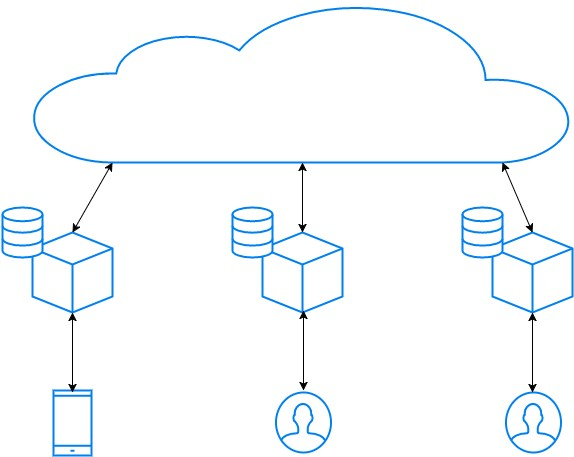
\includegraphics[width=\textwidth]{TraditionalArch}
\caption{Traditional Client-Proxy Architecture}
\end{figure}


In Figure 1 we can see a simple representation of the traditional role proxies have. Users connect to proxy servers as intermediaries to their connection to a network, such as the internet. Each of these proxies traditionally has its own disk and RAM cache. It is also possible to utilize these proxies as a distributed network with a shared cache represented by \lq joining \rq each of the disk caches into a unified cache. However, this cache still only incorporates the basic levels of disk and RAM storage and there is potentially significant overhead in communicating between proxies to locate content that may be on a different physical machine than the one handling the request and serving the content.





\section{Flying Squid}

\subsection{Apache Traffic Server}

Apache Traffic Server (ATS) is a high-performance open-source proxy that was built by Inktomi and Yahoo!. It is modular in nature, and is known for its efficient caching mechanisms. According to the ATS documentation, it \lq \lq is designed to improve content delivery for enterprises, ISPs, backbone providers, and large intranets by maximizing existing and available bandwidth \rq \rq \cite{ATS}.

Flying Squid is an Apache Traffic Server augmentation that can provide a distributed, cloud based cache localized at the edge of the network. The system utilizes custom caching techniques and protocols to reduce unnecessary bandwidth use. Thus, it provides faster data delivery than content providers by themselves. 

\begin{figure}[H] \centering
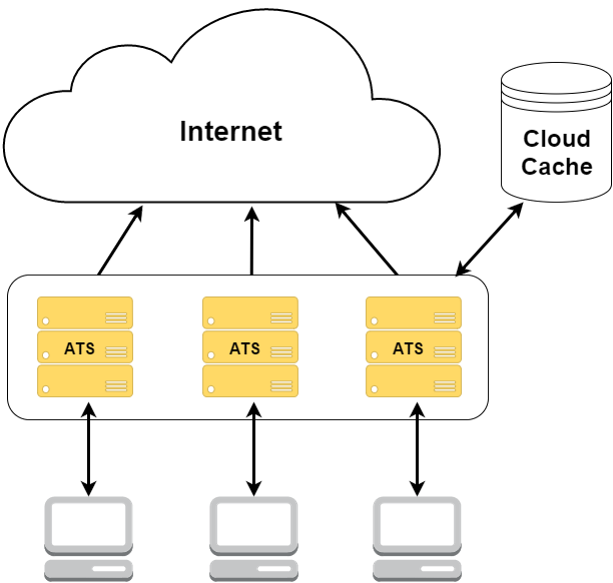
\includegraphics[width=\textwidth]{FlyingSquidArch}
\caption{Flying Squid Architecture}
\end{figure}


Flying Squid aims to be a truly web-based personal proxy, with shared cloud-based caches and value-based storage and transfer protocols. By improving content delivery speed and reducing client data usage, the proxy is especially useful to mobile users and those with spotty network connectivity.

\section{Cloud Caching}

FlyingSquid leverages different cloud storage tiers, each with unique benefits, to build a more sophisticated caching infrastructure. As a result, individual instances in an ATS cluster can be configured to share access to cached objects and use storage space more efficiently.

\begin{figure}[H] \centering
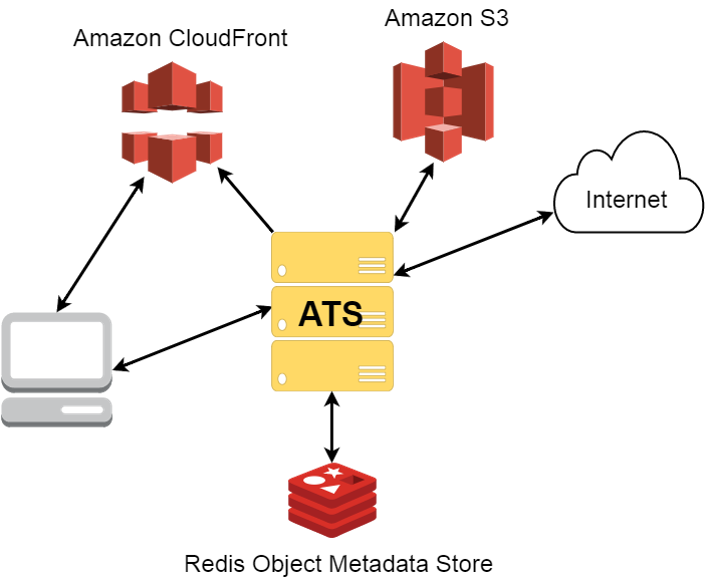
\includegraphics[width=\textwidth]{CloudCachingArch}
\caption{Flying Squid Proxy Cloud Caching Architecture}
\end{figure}

\subsection{Augmented Tier - Redis Cluster}
FlyingSquid uses a Redis in-memory key/value store to save HTTP object metadata. Each member of an ATS cluster has a master and slave pair of Redis instances. These instances are connected as a cluster and objects are stored across these instances according to how the cluster partitions keys. We chose to use this storage format for object metadata as opposed to storing data with each object because we needed a faster method of accessing data than querying S3 (where all cache objects are ultimately stored), as this type of query will inherently introduce significant performance penalties.

\newpage

\noindent
FlyingSquid uses the ATS computed cache key hash for each object as the key to store metatadata under and serialize the struct below to a string to store it in Redis.\\

\begin{lstlisting}
struct ObjectCacheMeta {
    int64_t size; // Object size in bytes
    int64_t headerLength;
    char *responseHeader; // Response header to send back to client
    long lastAccessed; // Unix timestamp of when object was last accessed
    long cloudFrontExpiry; // Unix timestamp of when object will be removed from CloudFront
  };
\end{lstlisting}

\noindent
Whenever we do a cache write we insert or update this object metadata. When we do cache reads and access objects in the cache, we update the lastAccessed timestamp and if applicable update the cloudFrontExpiry field.

\subsection{Storage Tier - AWS Simple Storage Service (S3)}
FlyingSquid utilizes Amazon S3 public cloud storage as the largest and slowest tier of the cloud cache. An ATS cluster is configured to share storage of HTTP objects in a S3 bucket. When ATS determines that an HTTP object is cacheable the object is uploaded to S3. When a cache read is called for we determine whether an object is in S3 from the Redis object metadata. If so, we simply retrieve it, collect the header from Redis, and send it back to the client.

\subsection{Storage Tier - AWS Cloudfront}
CloudFront is Amazon's Content Delivery Network service which can be utilized to push content to Amazon's servers at the edge of the network. FlyingSquid uses it to speed up object delivery to the client. When an object in the cache is deemed to be popular we set a field in its S3 metadata to push it to CloudFront. This field is equivalent to the HTTP \lq Expires \rq header and determines the lifetime of the object in this highest cache tier. When an object in CloudFront is requested by the client, an HTTP redirect is used to serve the response.


\section{Fingerprinting: Value Based Caching}

 Whether an application uses compression or intricate caching mechanisms, the easiest way to improve content delivery speed is to \textit{send less over the network}. With this in mind, a lot of research has been done with respect to protocols focused on eliminating redundant data transfers over HTTP links. Much of this redundancy is caused by the first-class nature of the \lq file \rq in traditional caching systems.\\

\noindent
Inspired by research at Berkley on value based caching\cite{Rhea09}, Flying Squid's Fingerprinting system caches with respect to data, not file name. As a result, only changed and new parts of content need ever retransmitted over a network. 


\subsection{The API}

Flying Squid's value based caching protocol takes the form of a simple, C++ class-based library. Modules exist on both the client and user side, and must be used together.

\subsubsection{Client}

\begin{lstlisting}
class RabinClient
{
    public:
        /* Server name and port number*/
        RabinClient(char * hostname, int port_);
       
	 ~RabinClient();

        /*
        * Receives a file from the server into the open, write enabled file pointer 'file'.
        * Returns the number of blocks added to the file.
	 * This is a blocking call.
        */
        unsigned receive_file(FILE *file); 

       /* Establishes a connection to the server */
        int connect_to_server();

	 /* Disconnects from the server */
        int disconnect_from_server();

};

\end{lstlisting}

\subsubsection{Server}

\begin{lstlisting}
class RabinServer
{

    public:
        /* Port at which to be open*/
        RabinServer(int port_);
        ~RabinServer();

        /* Sends a file of size s to the client.
		This is a blocking call.
	*/
        int send_file(char *file, size_t s); 


        /* Listens for the client and accepts a connection 
        * Must be called before write_to_client is called  */
        int connect_to_client();

	 /* Connects to the client */
        int disconnect_from_client();

};

\end{lstlisting}

\subsection{Integrating Value-Based Caching}

\noindent
Flying Squid uses modified TCP forwarding servers \cite{Partow} at both the client and server sides to interface value-based caching with ATS.

\begin{figure}[H] \centering
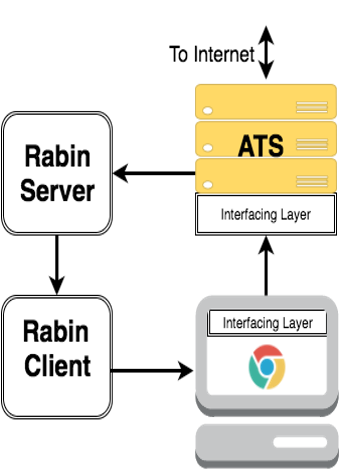
\includegraphics[width=9cm]{FingerprintingArch}
\caption{Flying Squid Value Based Caching Architecture}
\end{figure}

\noindent
When the user makes a request through the browser, the browser forwards the request through its interfacing layer to the interfacing layer of ATS. ATS receives this request and gathers the requested data file from the Internet and the cloud caching mechanism previously described. ATS then sends over the file to the Rabin Server, which breaks down the file into blocks. The Rabin Server sends each block to the Rabin Client, which reassembles the blocks into a file. The Rabin Client then sends the response to the browser through the browser's interfacing layer. Lastly, the browser displays the response to the user. 

\subsection{Technical Approach}

Flying Squid's Rabin Fingerprinting library provides a clean file transfer abstraction to the user, hiding the intricacies of a partial file transfer abstraction.

\begin{enumerate}

\item Server-side files are split into blocks of maximum size $1 KB$ using a \verb|djb-2|\cite{djb2} based uniform random function of the form: \\
$f: \{\text{byte} * \text{byte} * \text{byte} \} \rightarrow \{0, 1, ..., 1023\}$
 
\item Block boundaries are determined when this function returns 0. These blocks are treated as first-class objects and are hashed locally. A custom protocol can then be used to transfer the blocks representing a file over a TCP connection. Only the hash digests (identifiers) of previously transmitted blocks are transferred. Blocks of size 0 are used to denote $EOF$.

\item The client  leverages the ordering properties of TCP to receive blocks in order. These are then locally stored, and identifiers are used to re-assemble them into traditional files. 
\end{enumerate}

\subsection {Statistics}

Pairs of files were generated that differ in the following ways:

\begin{enumerate}
\item Haskell: One file has an added byte.
\item HTML: Files differ by one large contiguous chunk.
\item C: Files differ by a large number of chunks distributed through the file
\end{enumerate}

For each pair, these pairs of files were sent one after the other over a network using the Flying Squid fingerprinting system, with different maximum block sizes. Max block sizes 	smaller than $256$ bytes were found to cause significantly more conflicts with the internal \verb|djb2| hash. 


\begin{figure}[H] \centering
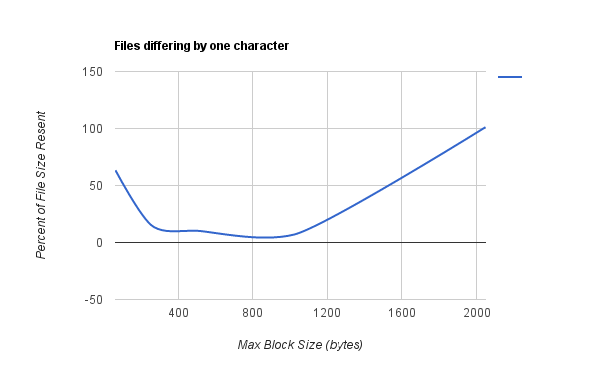
\includegraphics[width=\textwidth]{HaskellGraph.png}
\caption{Details the percent of the second file sent at different max block sizes.}
\end{figure}
\noindent
For files differing by one byte, a balance has to be struck between several small block headers being sent and the size of the retransmitted block(s). At most one block will be retransmitted due to the small difference between files. An optimal block size was found around $1000$ bytes

\begin{figure}[H] \centering
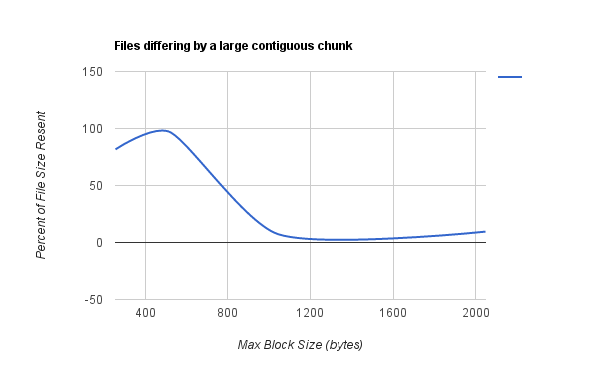
\includegraphics[width=\textwidth]{HTMLGraph.png}
\caption{Details the percent of the second file sent at different max block sizes.}
\end{figure}
\noindent
For files differing by a large contiguous chunk a minimum was found around $1400$ bytes.

\begin{figure}[H] \centering
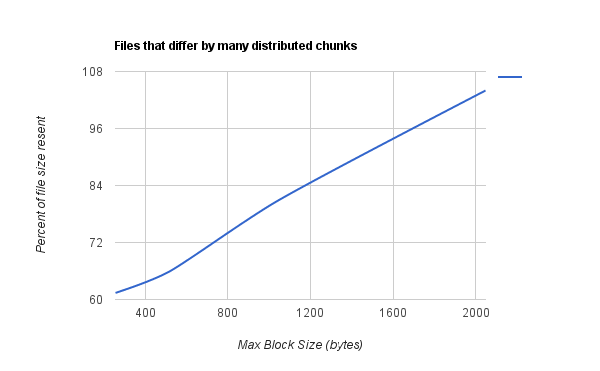
\includegraphics[width=\textwidth]{CGraph.png}
\caption{Details the percent of the second file sent at different max block sizes.}
\end{figure}
\noindent
For files differing by a large number of chunks distributed through the file, smaller max block sizes were generally found to be better.


\begin{figure}[H] \centering
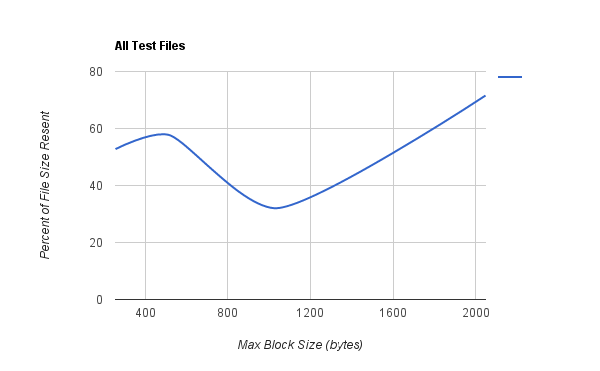
\includegraphics[width=\textwidth]{AllGraph.png}
\caption{Details the percent of the second file sent at different max block sizes.}
\end{figure}
\noindent
Taking the average of all these files, it was found that a minimal amount was resent around a maximum block size of $1 KB$. As a result, the maximum value chosen was $1024$ bytes, with an expected max size of $512$ bytes.



\section{Open Source Component}

We have been working with an open source fork of ATS hosted in our GitHub organization. The modifications we have made to ATS will hopefully be proposed as pull requests we can make to the main project. Several of our contributions have been placed directly in the ATS codebase. Thus, all modifications are open source contributions that we hope to be approved as part of the main Traffic Server codebase. 

The \lq Rabin \rq fingerprinting component of the project is also open source. It functions ias a standalone module that can be easily included in C++ code bases.

All of our GitHub repositories can be found at \url{https://github.com/FlyingSquid/}.

\section{Further Work}

A lot of work needs to be done to make Flying Squid a production level proxy system. The proxy is only as strong as its weakest link. The integration of cloud caches, ATS and fingerprinting systems could be further streamlined. Better integration would involve more robust browser-side clients, and the elimination of redundant actions within ATS. Value based caching could be made more flexible, with adjustable block sizes and less persistent TCP connections. More benchmark and bandwidth analysis could help better understand the strengths and weaknesses of Flying Squid. Eventually, this analysis would provide grounds for interesting research.

To accurately measure the effectiveness and relevance of Flying Squid, we must investigate several use cases for our proxy server. We must leverage these use cases to show, with measurable benchmarks, that Flying Squid is indeed an improvement on the proxy status quo. First, there is the use case of a proxy network with multiple nodes to maximize personalized caching for more than just an individual. The custom caching could cater to a corporation, non-profit organization, as well as universities like Tufts. 
Many countries in the world have extremely limited bandwidth. We must account for these use cases, as these countries’ population constitute a significant part of the world’s internet users. In effect, Flying Squid will deliver content to these users at speeds faster than the speed that is currently available.


\section{Conclusion}







\pagebreak

\begin{appendices}

\section{User Manual}

\subsection{Apache Traffic Server}

To run barebones, non-augmented version of ATS, run the following commands:

\begin{enumerate}

\item Clone the FlyingSquid scripts repository

\begin{lstlisting} [language=bash] 
git clone https://github.com/FlyingSquid/scripts.git
\end{lstlisting}

\item Change into the setup directory and execute the setup script.

\begin{lstlisting} [language=bash] 
cd ./scripts/setup
./setup.sh
\end{lstlisting}

This script installs the required dependencies, downloads trafficserver (ATS) into \verb|/mnt|, makes trafficserver, and installs it into \verb|/opt/ts|.

\item

Change into the traffic server directory and start Apache Traffic Server in debug mode (stoppable by \verb|Ctrl-C|):

\begin{lstlisting} [language=bash] 
sudo /opt/ts/bin/traffic_server
\end{lstlisting}

To start or stop trafficserver as a daemon process:
\begin{lstlisting}[language=bash]
sudo /opt/ts/bin/trafficserver stop
sudo /opt/ts/bin/trafficserver start
\end{lstlisting}

\item Make some changes to the ATS proxy configurations file to set it up as a forward proxy:

\begin{lstlisting} [language=bash] 
cd /opt/ts/etc/trafficserver
\end{lstlisting}

Open the \verb|records.config| file and replace the following lines:

\begin{verbatim}
CONFIG proxy.config.reverse_proxy_enabled INT 1
CONFIG proxy.config.url_remap.remap_required INT 1
CONFIG proxy.config.http.cache.http INT 0
\end{verbatim}

With the following lines:

\begin{verbatim}
CONFIG proxy.config.reverse_proxy_enabled INT 0
CONFIG proxy.config.url_remap.remap_required INT 0
CONFIG proxy.config.http.cache.http INT 1
\end{verbatim}

\item Test the proxy with the following command:

\begin{lstlisting} [language=bash] 
curl —-proxy http://127.0.0.1:8080 -o /dev/null http://i.imgur.com/A2FUg9g.png
\end{lstlisting}

\item To view the logging, execute the following command:

\begin{lstlisting} [language=bash] 
/opt/ts/bin/traffic_logcat -f /opt/ts/var/log/trafficserver/squid.blog
\end{lstlisting}

Additionally, ATS can be started with the debug mode to view any logs with a given tag

\begin{lstlisting}[language=bash]
sudo /opt/ts/bin/traffic_server -T<DEBUG_TAG>
\end{lstlisting}


\end{enumerate}

\subsection{ATS with Cloud Caching}

\begin{enumerate}

\item
Download and install the AWS C++ SDK

\begin{lstlisting}[language=bash]
cd /mnt
git clone https://github.com/aws/aws-sdk-cpp.git
mkdir build-aws-sdk-cpp
cd build-aws-sdk-cpp
cmake ../aws-sdk-cpp -DBUILD_ONLY="aws-cpp-sdk-s2" -DCUSTOM_MEMORY_MANAGEMENT=0
make
sudo make install
\end{lstlisting}

\item
Point ATS cache Makefile to the local version of the headers:

Open \verb|/mnt/trafficserver/iocore/cache/Makefile.am| and update line 31 and 32 to reflect where your AWS C++ SDK headers reside. Most likely, they will be updated to the following:

\begin{verbatim}
-I/mnt/aws-sdk-cpp/aws-cpp-sdk-core/include \
-I/mnt/aws-sdk-cpp/aws-cpp-sdk-s3/include
\end{verbatim}

\item
Update the following lines in \verb|/opt/ts/etc/trafficserver/records.config|

\begin{verbatim}
CONFIG proxy.config.http.cache.cloud.enable INT 0
CONFIG proxy.config.http.cache.cloud.provider STRING NULL
\end{verbatim}

To the following to enable cloud caching with AWS:

\begin{verbatim}
CONFIG proxy.config.http.cache.cloud.enable INT 1
CONFIG proxy.config.http.cache.cloud.provider STRING "aws" 
\end{verbatim}

\item
Install the Redis command line interface from: \url{http://redis.io/download}

Set up an initial cluster with the following tutorial:

 \url{http://redis.io/topics/cluster-tutorial}

\item
Recompile ATS and run:

\begin{lstlisting}[language=bash]
cd /mnt/trafficserver
make && sudo make install
sudo /opt/ts/bin/traffic_server
\end{lstlisting}

\end{enumerate}

\subsection{Value-Based Caching Integration}

To run Flying Squid, run the following commands in the following order:

\begin{enumerate}

\item 

\begin{lstlisting} [language=bash] 
sudo /opt/ts/bin/trafficserver start
\end{lstlisting}

ATS will be running on port 8080.

\item 

Set Google chrome or Mozilla Firefox to point to the port that the TCP Proxy Client (Browser's Interfacing Layer) will run on. 

\item 

Start up the TCP Proxy Server (ATS's Interfacing Layer) in another terminal:

\begin{lstlisting} [language=bash] 
cd $(RABIN_FINGERPRINT_DIR)/Integration/tcpproxy
tcpproxy_server <local host ip> <tcpproxy_server port> <local host ip> 8080
\end{lstlisting}

\item

Start up the TCP Proxy Client (Browser's Interfacing Layer) in another terminal:

\begin{lstlisting} [language=bash] 
cd $(RABIN_FINGERPRINT_DIR)/Integration/tcpclient.
tcpproxy_client <local host ip> <tcpproxy_client port> <local host ip> <tcpproxy_server port>
\end{lstlisting}

\item

Open the browser that is pointing to the TCP Proxy Client and make request to a website, e.g. http://www.cs.tufts.edu.

\end{enumerate}

\subsection{Rabin Fingerprinting Demo}

\begin{enumerate}

\item 

Start up the Rabin Fingerprinting Server:

\begin{lstlisting} [language=bash] 
cd $(RABIN_FINGERPRINT_DIR)/Server
./rabinserver <Rabin Server port> ../Files/HTML/CSWebpage.html ../Files/HTML/CSWebpageWithoutHead.html
\end{lstlisting}

\item Start up the Rabin Fingerprinting Client in another terminal:

\begin{lstlisting} [language=bash] 
cd $(RABIN_FINGERPRINT_DIR)/Client
./rabinclient localhost <Rabin Server port> test.html
\end{lstlisting}

\end{enumerate}



\section{Better Integration: Google Native Client \cite{Google Native Client}}

\paragraph{Idea}

The idea behind using Google Native Client is simply to eliminate the browser's interfacing layer. With Google Native Client, the browser can run C++ code in the browser. This way, the request does not have to pass through the TCP proxy interfacing layer and can go straight to ATS. Not only would this make Flying Squid more secure and portable, but it would also bring huge performance benefits.

In a web application, Google Native Client is embedded within the HTML through the use of an <embed> tag. The JavaScript and Google Native Client modules talk to each other via bidirectional, asynchronous messages.

\paragraph{Setting up Native Client}

Before Native Client can be set up, Python 2.7 and Make need to be available on the machine. Once these executables are available, the Native Client executable can be downloaded at the following website: https://developer.chrome.com/native-client/sdk/download. A Hello World Tutorial is also available at https://developer.chrome.com/native-client/devguide/tutorial/tutorial-part1.

For our purposes, however, perform the following steps to get up to speed:

\begin{enumerate} 
\item Clone the clientInterfacing directory. The command is 

\begin{lstlisting} [language=bash] 
git clone https://github.com/FlyingSquid/clientInterfacing.git
\end{lstlisting}

\item  Make sure your Google Chrome browser is version 49 or higher.

\item Change into the directory nacl_sdk/pepper_49/getting_started/part1.

\item Execute \lq make \rq .

\item Change into the directory nacl_sdk/pepper_49/getting_started.

\item Execute \lq make serve \rq .

\item Use the Google Chrome browser to access http://localhost:5103. 

\end{enumerate}

\paragraph{Debugging}

The application can also be opened on MAC OSX in the terminal via the following commands:

\begin{lstlisting} [language=bash]
mkdir ~/Desktop/testtest

cd /Applications/Google Chrome.app/Contents/MacOS

./Google\ Chrome http://localhost:5103/part1 --enable-logging --v=1 --user-data-dir=~/Desktop/testtest
\end{lstlisting}

This will enable logging to appear, making it easier for future developers to debug the Native Client module.


\paragraph{Challenges}

Unfortunately, there were a few roadblocks that prevented Google Native Client from being a viable option for Flying squid at the moment. The roadblocks are listed below and are left for future developers to tackle.

\begin{enumerate}

\item Google Native Client cannot be compiled with g++ and the -std=c++0x flag, both of which are required to compile the Rabin Client and Rabin Server correctly. 

\item Google Native Client cannot access the local filesystem of the machine that it is running on. It can only simulate a File I/O API using a ocal secure data store. This File I/O API is described here: https://developer.chrome.com/native-client/devguide/coding/file-io. Further documentation of implementations of standard POSIX I/O functions such as fopen, fseek, fread, fwirte, and fclose are described here: https://developer.chrome.com/native-client/devguide/coding/nacl_io.

\end{appendices}

\printbibliography

\end{document}